\chapter{Theorie}

\section{Neuronales Netzwerk}
In diesem Abschnitt der Arbeit wird der Aufbau eines neuronalen Netzwerks näher betrachtet und entsprechend auf die Terminologie in diesem Bereich eingegangen. \\
Neuronale Netzwerke sind den biologischen Neuronen nachempfunden und setzen sich daher aus Vielzahl von Neuronen zusammen. Darüber hinaus ist ein Netzwerk in mehrere Schichten untergliedert (siehe Abb.\ref{fig:neural_network_extended}). So wird die erste Schicht auf der linken Seite auch als \textit{Eingabeschicht} und alle korrespondierenden Eingabeknoten als Eingabeneuron bezeichnet. Die letzte Schicht, die sogenannte \textit{Ausgabeschicht}, beinhaltet dagegen alle \textit{Ausgabeneuronen}. Alle Schichten zwischen der Eingabe und der Ausgabe tragen die Bezeichnung des \textit{Hidden Layer}, wobei ein Netzwerk mehrere dieser Schichten aufweisen kann. In der folgenden Grafik ist ein 4-Layer-Netzwerk abgebildet, das zwei \textit{Hidden Layer} besitzt. Diese mehrschichtigen Netzwerke werden ebenfalls als \textit{Multilayer Perceptrons} oder \textit{MLPs} bezeichnet, obwohl das Netzwerk sich aus Sigmoid-Neuronen zusammensetzt.
\begin{figure}[hbt]
	\centering
	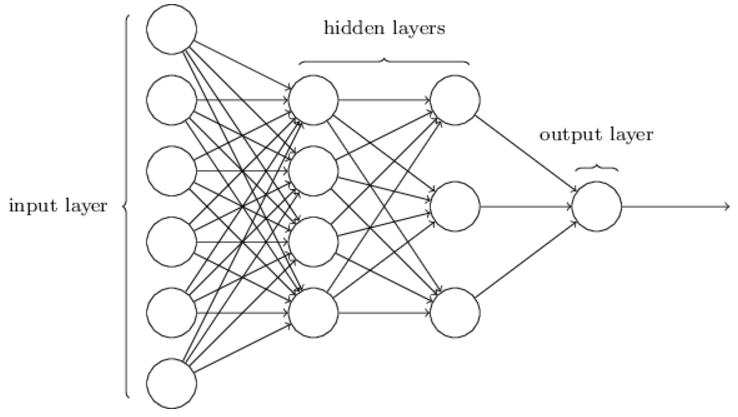
\includegraphics[scale=0.6]{Bilder/neural_network_extended}
	\caption{Aufbau des neuronalen Netzwerks hinsichtlich der einzelnen Layer.} 
	\label{fig:neural_network_extended} 
\end{figure}

\noindent
Für die Zusammensetzung von Eingabe- und Ausgabeschichten in einem Netzwerk, fällt die Betrachtung auf die Erkennung einer handgeschrieben "9". Als Eingabewerte dienen dem Netzwerk die Intensitäten der Bildpixel. Liegt ein Graustufenbild der Größe von 64x64 Pixeln vor, leiten sich daraus 4096 Eingabeknoten  mit skalierten Intensitätswerten zwischen 0 und 1 ab. Die Ausgabeschicht beinhaltet dagegen nur ein Neuron, um eine entsprechende Klassifizierung der "9" vornehmen zu können. \\[0.2cm]
\hspace*{1.3cm}
$ 
\begin{array}[t]{lcll}
	\mathtt{output} < 0.5 \quad\rightarrow\quad \mbox{"Eingabebild ist keine 9"} \\[0.2cm]
	\mathtt{output} \geq 0.5 \quad\rightarrow\quad \mbox{"Eingabebild ist eine 9"}
\end{array}
$
\\[0.2cm]
Im Vergleich hierzu ist der Aufbau der Hidden-Layer nicht durch irgendwelche Regeln ableitbar. Zum Einsatz kommen Heuristiken, die das Verhalten eines Netzwerkes bestimmen, welches ausgehend vom Experiment erwartet und gewünscht wird. Zum Beispiel kann untersucht werden, wie die Lernrate des Netzwerks sich im Verhältnis zu der Anzahl an Hidden-Layer verhält. \\

\noindent
Bisher fiel die Betrachtung in dieser Arbeit auf neuronale Netze, bei denen die Ausgabe einer Schicht die Eingabe in der nächsten Schicht darstellte. Solche Netzwerke werden auch \textit{Feedforward Neural Networks} bezeichnet. Hierunter ist das nicht Auftreten von Schleifen zu verstehen - sprich, Informationen werden im Netzwerk immer von Layer $n$ zu Layer $n+1$ übergeben. Somit kann verhindert werden, dass das Netzwerk in gewissen Fällen bei der Eingabe der Sigmoid-Funktion $\sigma$ von dessen Ausgabe abhängig ist. \\
Ebenfalls gibt es Netzwerke bei denen sogenannte \textit{Feedback Loops} möglich sind. In diesem Fall handelt es sich um \textit{Recurrent Neural Networks}. Die Idee hinter diesem Modell ist, dass bestimmte Neuronen über einen definierten Zeitraum aktiv sind bevor sie inaktiv werden. Dies kann andere Neuronen anregen, ebenfalls über einen gewissen Zeitraum aktiv zu sein und eine entsprechende Kettenreaktion auslösen (Kaskade). Schleifen stellen in diesem Modell kein Problem dar, da die Ausgabe eines Neurons erst zu einem späteren Zeitpunkt die Eingabe beeinflusst. \\
Stellt man diese Arten von neuronalen Netzwerken gegenüber, so lässt sie zum heutigen Zeitpunkt die Aussage treffen, dass Feedback Neural Networks weniger Verbreitung finden. Dies ist begründet in der Leistungsfähigkeit der Lernalgorithmen. Jedoch sollte an dieser Stelle berücksichtigt werden, dass mittels Feedback Neural Networks bestimmte Probleme mit einem geringeren architektonischen Aufwand gelöst werden können. Darüber hinaus bildet der komplexere logische Aufbau eines solchen Netzwerks das menschliche Verhalten besser ab.

\section{Perceptrons}
Ein Perceptron ist ein mathematisches Modell zur Abbildung eines künstliches Neurons in einem Netzwerk. Es wird für die Entscheidungsfindung herangezogen, indem verschiedene Aussagen abgewägt werden. Hierbei nimmt das Perceptron eine Menge von Eingaben $x_n$ mit $n \in \{1, \cdots, m\}$ und berechnet einen einzigen binären Ausgabewert (siehe Abb. \ref{fig:perceptron}). 
\begin{figure}[hbt]
	\centering
	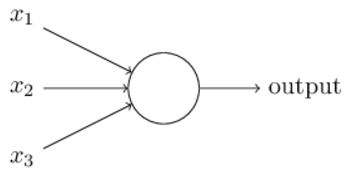
\includegraphics[scale=0.6]{Bilder/perceptron}
	\caption{Percetron mit den Eingaben $x_1, x_2, x_3$ und der Ausgabe $\mathtt{output}$.} 
	\label{fig:perceptron} 
\end{figure}

\noindent
Für jeden Eingabewert $x_n$ wird eine Gewichtung $w_n$ mit $n \in \{1, \cdots, m\}$ zugeordnet. Der Ausgabewerte $\mathtt{output}$ wird mittels der gewichteten Summe $\sum_j w_j x_k$ und einem definierten Grenzwert $\mathtt{threshold}$ bestimmt.
\begin{equation}
	\mathtt{output} := \left\{
	\begin{array}{ll}
 		0 & \displaystyle \mbox{falls}\quad \sum\limits_j w_j x_j \leq \mathtt{threshold} \\[0.5cm]
 		1 & \displaystyle \mbox{falls}\quad \sum\limits_j w_j x_j > \mathtt{threshold}
	\end{array}\right.
\end{equation}

\noindent
Der Aufbau des Netzwerks leitet sich aus den unterschiedlichen Modellen der Entscheidungsfindung ab und wird mit Hilfe der Perceptrons abgebildet (siehe Abb. \ref{fig:perceptron_models}).
\begin{figure}[hbt]
	\centering
	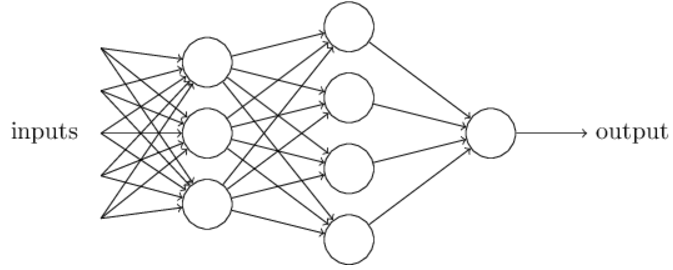
\includegraphics[scale=0.75]{Bilder/perceptron_models}
	\caption{Unterschiedliche Möglichkeiten der Entscheidungsfindung.} 
	\label{fig:perceptron_models} 
\end{figure}
Eine Entscheidungsmöglichkeit wird hierbei durch das Perceptron dargestellt. Weiterhin wird eine Spalte von Perceptrons als Schicht bezeichnet. Die erste Schicht fällt Entscheidungen auf Gewichtung der Eingabewerte, indem er diese abwägt. Jedes Perceptron der zweiten Schicht hingegen, wägt für die Entscheidungsfindung die Resultate der ersten Schicht ab. Ein Perceptron auf der zweiten Schicht kann somit eine Entscheidung auf einer abstrakteren und komplexeren Ebene durchführen. Auf diese Weise kann sich ein vielschichtiges Netzwerk von Perceptrons in ein anspruchsvolles Modell zur Entscheidungsfindung entwickeln. \\

\noindent
Im folgenden wird die mathematische Beschreibung von Perceptrons vereinfacht, indem Änderungen an der Notation für $\sum_j w_j x_j > \mathtt{threshold}$ vorgenommen werden. Für die Beschreibung der Summe $\sum_j w_j x_j$ werden die Vektoren $\mathbf{w}$ und $\mathbf{x}$ eingeführt, wodurch sich die Schreibweise $\mathbf{w} \cdot \mathbf{x} \equiv \sum_j w_j x_j$ ergibt. Des Weiteren wird der $\mathtt{threshold}$ auf die andere Seite der Ungleichung gezogen und erhält die Bezeichnung \textit{Vorbelastung}, $b \equiv \mathtt{-threshold}$. 
\begin{equation}
	\mathtt{output} := \left\{
	\begin{array}{ll}
 		0 & \displaystyle \mbox{falls}\quad \mathbf{w} \cdot \mathbf{x} + b \leq 0 \\[0.2cm]
 		1 & \displaystyle \mbox{falls}\quad \mathbf{w} \cdot \mathbf{x} + b > 0
	\end{array}\right.
\end{equation}

\noindent
Dieses mathematische Verhalten wird durch die folgende Stufenfunktion verdeutlicht (siehe Abb. \ref{fig:perceptron_plot}).
\begin{figure}[hbt]
	\centering
	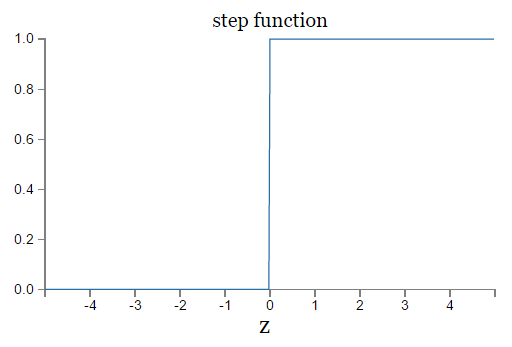
\includegraphics[scale=0.6]{Bilder/perceptron_plot}
	\caption{Sigmoid Funktion $\sigma(z)$.} 
	\label{fig:perceptron_plot} 
\end{figure}

\section{Arbeitsweise von Perceptrons}
Ein einzelnes Perceptron kann für die Darstellung unterschiedlicher boolescher Funktionen genutzt werden. Angenommen die Definition der booleschen Werte 1 ($\mathtt{true}$) und 0 ($\mathtt{false}$) liegt zugrunde, so ist es möglich alle logische Operationen z.B. $\mathtt{AND}$, $\mathtt{OR}$ und $\mathtt{NAND}$ über ein Perceptron abzubilden. \\
Im weiteren Verlauf soll die Umsetzung eines $\mathtt{NAND}$ Gatters mit Perceptrons betrachtet werden. $\mathtt{NAND}$ Gatter spielen in der Digitaltechnik eine bedeutende Rolle, da sie alle logischen Verknüpfungen und somit auch komplexere Schaltungen (z.B. Addierer, Multiplexer) zusammenstellen lassen. Fällt die Betrachtung auf ein Perceptron mit 2 Eingaben deren Gewichtung jeweils den Wert -2 aufweisen und eine Vorbelastung von 3, so ergibt sich folgende Abbildung (siehe Abb. \ref{fig:perceptron_example}).
\begin{figure}[hbt]
	\centering
	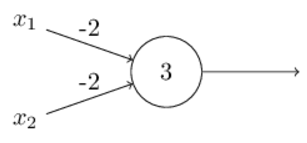
\includegraphics[scale=0.6]{Bilder/perceptron_example}
	\caption{Percetron mit zwei Eingaben -2 und einem Bias von 3.} 
	\label{fig:perceptron_example} 
\end{figure}

\noindent
Um das Verhalten des Perceptrons weiter zu untersuchen werden zum einen die Eingaben $x_1, x_2$  mit dem Wert 0 und zum anderen mit dem Wert -1 belegt. \\[0.2cm]
\hspace*{1.3cm}
$
\begin{array}[t]{lclll}
	(-2)*0+(-2)*0+3 & = & 3 & \geq & 0  \quad\rightarrow\quad \mathtt{output} := 1 \\[0.2cm]
	(-2)*1+(-2)*1+3 & = & -1  & < & 0 \quad\rightarrow\quad \mathtt{output} := 0
\end{array}
$
\\[0.2cm]
Das vorliegende Perceptron ist in der Lage das Verhalten eines $\mathtt{NAND}$ Gatters nachzubilden. Somit kann auf dessen Basis auch ein Halbaddierer, der die Addition von zwei Bits $x_1$ und $x_2$ durchführt, implementiert werden. Für die Berechnung wird die bitweise Summe $x_1 \oplus x_2$ gebildet, wobei ein $\mathtt{carry bit}$ den Wert 1 annimmt, sobald $x_1$ und $x_2$ den Wert 1 aufweisen.
\begin{figure}[hbt]
	\centering
	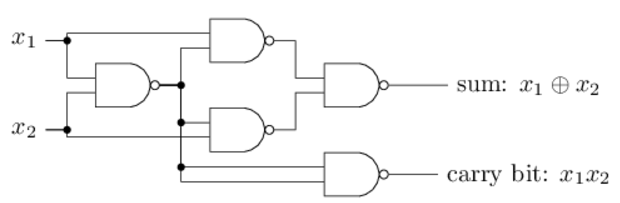
\includegraphics[scale=0.6]{Bilder/nand_gatter}
	\caption{Halbaddierer mit den Eingaben $x_1$ und $x_2$.} 
	\label{fig:nand_gatter} 
\end{figure}

\noindent
Um ein gleichwertiges Netzwerk abzuleiten, werden die $\mathtt{NAND}$ Gatter durch Perceptrons mit jeweils 2 Eingaben ersetzt. Hierbei weisen die Gewichtungen $w_1, w_2$ den Wert -2 und die Vorbelastung $b$ den Wert 3 auf. 
\begin{figure}[hbt]
	\centering
	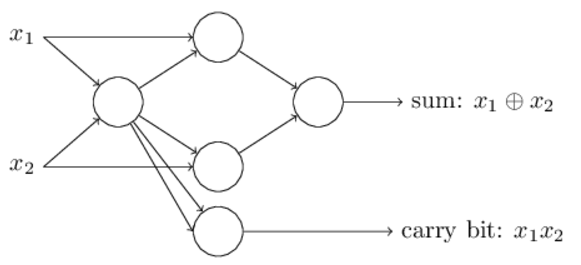
\includegraphics[scale=0.6]{Bilder/nand_gatter_perceptron}
	\caption{Halbaddierer-Aufbau mit Perceptrons.} 
	\label{fig:nand_gatter_perceptron} 
\end{figure}

\noindent
In einem weiteren Schritt wird die Abbildung eines $\mathtt{NAND}$ Gatter mit Perceptrons vereinfacht. Dazu werden mehrere Eingänge eines Perceptrons zu einem zusammengefasst, weshalb aus den zwei Eingaben -2 der Wert -4 resultiert. Ebenfalls werden die Eingaben in der Eingabeschicht des neuronalen Netzwerkes zusammengefasst, wobei jedoch durch diese Notation eine Eingabe nicht mit einem Perceptron gleichzustellen ist. Das vorliegende Netzwerk mit Perceptrons entspricht somit dem Aufbau eines Halbaddierers (siehe Abb. \ref{fig:nand_gatter_perceptron_simplified}). \\
\begin{figure}[hbt]
	\centering
	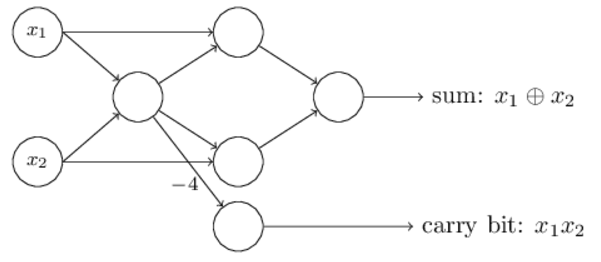
\includegraphics[scale=0.6]{Bilder/nand_gatter_perceptron_simplified}
	\caption{Vereinfachter $\mathtt{NAND}$ Gatter Aufbau mit Perceptrons.} 
	\label{fig:nand_gatter_perceptron_simplified} 
\end{figure}

\noindent
Wie im obigen Beispiel aufgezeigt, lassen sich mittels Perceptrons unterschiedliche Berechnungen durchführen. Auf diese Weise können implementierte Lernalgorithmen Gewichtungen sowie die Vorbelastung automatisch durch entsprechende Stimuli im Netzwerk anpassen und ermöglichen die Nutzung von künstlichen Neuronen.

\section{Sigmoid Neurons}
Für die Entwicklung lernender Algorithmen in einem Netzwerk, fällt die Betrachtung in dieser Arbeit auf die Erkennung von handgeschrieben Zahlen. Die Eingabe für das Netzwerk könnten die Raw Pixeldaten der eingescannten Bilder darstellen, welche die handgeschrieben Zahlen abbilden. Das Ziel an dieser Stelle ist, dass das Netzwerk anhand der Veränderungen von \textit{Gewichtungen} und der \textit{Vorbelastung} lernt eine korrekte Klassifizierung der Zahlen vorzunehmen. \\
Das Modifizieren der \textit{Gewichtungen} und der \textit{Vorbelastung} von Neuronen kann das Verhalten des Netzwerkes und deren Entscheidungsfindung zu Problemen beeinflussen. Angenommen die Erkennung und Klassifizierung einer Zahl wurde durch das Netzwerk falsch vorgenommen, so können durch kleine Veränderungen an den \textit{Gewichtungen} und der \textit{Vorbelastung} eine Korrektur durchgeführt werden. Dieses stetige Modifizieren der Werte über einen definierten Zeitraum ermöglicht ein lernendes Netzwerk (siehe Abb. \ref{fig:sigmoid_learning}). 
\begin{figure}[hbt]
	\centering
	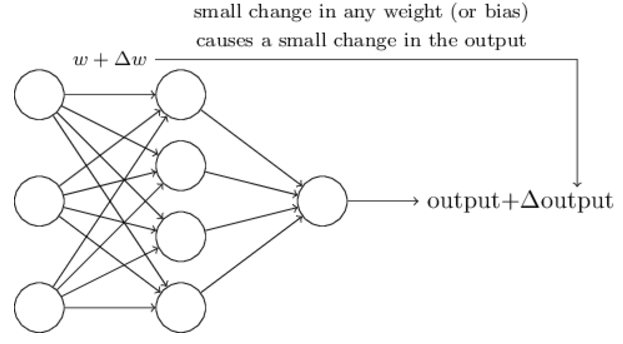
\includegraphics[scale=0.7]{Bilder/sigmoid_learning}
	\caption{Modifizieren von Weights und Biases schaffen lernendes Netzwerk.} 
	\label{fig:sigmoid_learning} 
\end{figure}

\noindent
Mit Hilfe der Einführung des Sigmoid Neurons soll der Fehler zur Klassifizierung von Zahlenwerten minimiert werden. Eine Änderung der Gewichtungen und der Vorbelastung bei diesem künstlichen Neuron soll nur marginale Änderungen an dem Ausgabewert $\mathtt{output}$ vornehmen. Diese Erweiterung des Neurons begünstigt ein Netzwerk selbständig die Klassifizierung von Zahlen zu optimieren. \\[0.2cm]
\hspace*{1.3cm}
$
\begin{array}[t]{lclll}
	\mathbf{w} + \Delta\mathbf{w} \quad\rightarrow\quad \mathtt{output} + \Delta\mathtt{output}
\end{array}
$
\\[0.2cm]

\noindent
Der Aufbau des Sigmoid Neurons ähnelt dem Perceptron, wobei das Neuron eine Anzahl von Eingabewerten $x_n$ mit $n \in \{1, \cdots ,m\}$ entgegennimmt und ausgehend von diesen Informationen den $\mathtt{output}$ ermittelt. Der wesentliche Unterschied zwischen diesen zwei Typen von Neuronen liegt in der differenzierbaren Funktion des Sigmoid Neurons zur Bestimmung des Ausgabewertes. Bei dem Sigmoid Neuron kann dieser alle Werte im Intervall $[0,1]$ annehmen. Weiterhin weist auch diese Art von Neuronen für jeden Eingabewert eine Gewichtung $w_n$ mit $n \in \{1, \cdots ,m\}$ sowie eine Vorbelastung auf. \\
Für die Berechnung des $\mathtt{output}$ wird in diesem Kontext die \textit{Sigmoid Funktion} $\sigma(z)$ angewendet.
\begin{equation}
	\sigma(z) \equiv \frac{1}{1+e^{-z}} \quad\mbox{mit}\quad z = \mathbf{w} \cdot \mathbf{x} + b
\end{equation}
Unter Berücksichtigung des Gewichtungsvektors \\[0.2cm]
\hspace*{1.3cm}
$
\begin{array}[t]{lclll}
	\mathbf{w} = \langle w_1, \cdots, w_m \rangle^\top
\end{array}
$
\\[0.2cm]
und des Eingabevektors \\[0.2cm]
\hspace*{1.3cm}
$
\begin{array}[t]{lclll}
	\mathbf{x} = \langle x_1, \cdots, x_m \rangle^\top
\end{array}
$
\\[0.2cm]
ergibt sich mit der Indexnotation 
\begin{equation}
	\sigma(z) \equiv \frac{1}{1+\exp(-\sum_j w_j x_j - b)}.
\end{equation}
Dabei weist das Sigmoid Neuron das gleiche Verhalten wie ein Perceptron auf, wenn eine Grenzwertbetrachtung durchführt wird. \\[0.2cm]
\hspace*{1.3cm}
$
\begin{array}[t]{lcll}
	\lim\limits_{z \to \infty}{\sigma(z)} & \approx & 1 \quad\quad bzw. \\[0.2cm]
	\lim\limits_{z \to -\infty}{ \sigma(z)} & \approx & 0
\end{array}
$
\\[0.2cm]
Dieses Verhalten wird weiterhin verdeutlicht, wenn die Betrachtung auf den folgenden Funktionsgraph fällt (siehe Abb. \ref{fig:sigmoid_plot}). Für große $z$ nimmt die Funktion den Wert 1 an und für kleine $z$ nimmt die Funktion den Wert 0 an.
\begin{figure}[hbt]
	\centering
	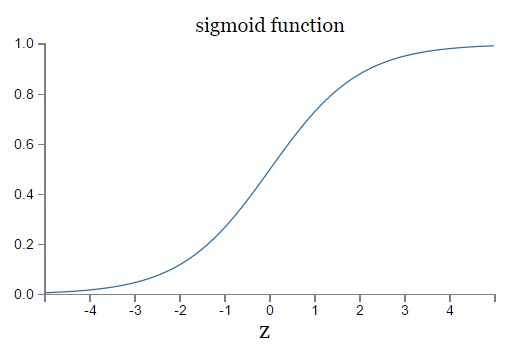
\includegraphics[scale=0.6]{Bilder/sigmoid_plot}
	\caption{Sigmoid Funktion $\sigma(z)$.} 
	\label{fig:sigmoid_plot} 
\end{figure}

\noindent
Die Vorteile der Sigmoid Funktion liegen in den marginalen Änderungen $\Delta w_j$ bei den Gewichtungen und $\Delta b$ bei der Vorbelastung, welche eine marginale Änderung am $\Delta\mathtt{output}$ vornehmen. Damit stellt $\Delta\mathtt{output}$ die lineare Funktion bezüglich der Änderungen  $\Delta w_j$ und $\Delta b$ in den Gewichtungen und der Vorbelastung dar.
\begin{equation}
	\Delta\mathtt{output} \equiv \sum_{j}{\frac{\partial\mathtt{output}}{\partial w_j}\Delta w_j+\frac{\partial\mathtt{output}}{\partial b}\Delta b}
\end{equation}
Diese Linearität begünstigt die Wahl von kleinen Änderungen in den Gewichtungen und der Vorbelastung, um das Verhalten für ein lernendes Netzwerk abzuleiten. \\

\noindent
Ein \textit{Feedforward Neural Network} besteht aus $L$ Schichten, wobei die Topologie des Netzwerkes durch $L \in \mathbb{N}$ und einer Liste $[m(1),\cdots ,m(L)]$ geben ist. $L$ bezeichnet die Anzahl der Schichten, während $m(l)$ mit $l \in \{2,\cdots ,L\}$ die Anzahl der Neuronen in der $l$-ten Schicht angibt. Somit ist erste Schicht des Netzwerks, die Eingabeschicht, über die Eingabedimension $m(1)$ und die Ausgabedimension über $m(L)$ definiert. \\
Jedes Neuron der $l$-ten Schicht hat über die Gewichtung eine Verbindung zu einem Neuron in der $(l+1)$-ten Schicht. Die Gewichtung $w_{j,k}^{(l)}$ stellt die Verbindung des $k$-ten Neurons in der $l-1$ Schicht zu dem $j$-ten Neuron in der $l$-ten Schicht. Die Gewichtungen in Schicht $L$ werden über die Gewichtungsmatrix $W^{(l)}$ der Schicht $l$ zusammengefasst. Die Matrix ist wie folgt definiert \\[0.2cm]
\hspace*{1.3cm}
$
\begin{array}[t]{lclll}
	W^{(l)} := \left( w_{j,k}^{(l)}\right)
\end{array}
$
\\[0.2cm]
und ist eine $m(l)\times m(l-1)$ Matrix, wobei \\[0.2cm]
\hspace*{1.3cm}
$
\begin{array}[t]{lclll}
	W^{(l)} \in \mathbb{R}^{m(l)\times m(l-1)}.
\end{array}
$
\\[0.2cm]
Weiterhin hat das $j$-te Neuron in Schicht $l$ eine Vorbelastung $b_j^{(l)}$. Die Vorbelastungen der Neuronen in Schicht $l$ werden über den Vorbelastungsvektor \\[0.2cm]
\hspace*{1.3cm}
$
\begin{array}[t]{lclll}
	\mathbf{b}^{(l)} := \langle b_1^{(l)},\cdots ,b_{m(l)}^{(l)}\rangle
\end{array}
$
\\[0.2cm]
zusammengefasst. Hieraus ergibt sich für das $j$-te Neuron der $l$-ten Schicht die Sigmoid Funktion $\sigma_j^{(l)}$, die wie folgt rekursiv definiert wird:
\begin{enumerate}
	\item Für die Eingabeschicht ergibt sich 
			\begin{equation}
        	\label{eq:feedforward1}
      			 \sigma_j^{(1)}(z) := x_j.
     		\end{equation}
    \item Für alle anderen Schichten ergibt sich
    		\begin{equation}
         	\label{eq:feedforward2}
         		\sigma_j^{(l)}(z) := 
             	\sum\limits_{k=1}^{m(l-1)} \left(w_{j,k}^{(l)}\cdot \sigma^{(l-1)}(z) + b_{j}^{(l)}\right) \quad \mbox{for all $l \in \{2, \cdots, L\}$}.
			\end{equation}
\end{enumerate}
Die Ausgabe des neuronalen Netzwerks für eine gegebene Eingabe $\mathbf{x}$ ist durch die Neuronen der Ausgabeschicht festgelegt. Diese werden über den Ausgabevektor $\mathbf{o} \in \mathbb{R}^{m(L)}$ mit \\[0.2cm]
\hspace*{1.3cm}
$
\begin{array}[t]{lclll}
	\mathbf{o}(x) := \langle \sigma_1^{(L)}(x),\cdots ,\sigma^{(L)}(z)\rangle = \sigma^{(L)}(x)
\end{array}
$
\\[0.2cm]
definiert. Unter Berücksichtigung der Gleichungen \ref{eq:feedforward1} und \ref{eq:feedforward2} kann nun nachvollzogen werden, wie Informationen das Netzwerk durchlaufen.
\begin{enumerate}
	\item  Der gegebene Eingabevektor $\mathbf{x}$ wird in der ersten und sogenannten Eingabeschicht des neuronalen Netzwerks gespeichert: \\[0.2cm]
\hspace*{1.3cm}
$
\begin{array}[t]{lclll}
	\sigma^{(1)}(z) := \mathbf{x}.
\end{array}
$
	\item Auf der zweiten Schicht liegt die erste Neuronenebene vor bei denen die Sigmoid Funktion zum Einsatz kommt: \\[0.2cm]
\hspace*{1.3cm}
$
\begin{array}[t]{lclll}
	\sigma^{(2)}(z) := W^{(2)}\cdot \sigma^{(1)}(z)+\mathbf{b}^{(2)} = W^{(2)}\cdot \mathbf{x}+\mathbf{b}^{(2)}.
\end{array}
$
\item Auf der dritten Schicht liegt die zweite Neuronenebene vor bei denen die Sigmoid Funktion zum Einsatz kommt: \\[0.2cm]
\hspace*{1.3cm}
$
\begin{array}[t]{lclll}
	\sigma^{(3)}(z) := W^{(3)}\cdot \sigma^{(2)}(z)+\mathbf{b}^{(3)} = W^{(3)}\cdot \left(W^{(2)}\cdot \mathbf{x}+\mathbf{b}^{(2)}\right)+\mathbf{b}^{(3)}.
\end{array}
$
\item Dieser Vorgang wird solange durchlaufen bis die Ausgabeschicht erreicht wird und die Ausgabe \\[0.2cm]
\hspace*{1.3cm}
$
\begin{array}[t]{lclll}
	\mathbf{o}(\mathbf{x}) := \sigma^{(L)}(z)
\end{array}
$
\end{enumerate}

\section{Stochastic Gradient Descent}
Für eine zuverlässige Klassifizierung der Zahlen wird ein Algorithmus benötigt, der die Bestimmung von Gewichtungen und der Vorbelastungen ...

\section{Backpropagation}

%\section{Netzwerk zur Klassifizierung von handgeschrieben Zahlen}
